\documentclass{article}
\usepackage{graphicx}
\usepackage{subcaption}
\usepackage{geometry}
 \geometry{
 a4paper,
 total={170mm,257mm},
 left=20mm,
 top=20mm,
 }

\title{Assignment 3 - Part 3.1: 2D Manifold \\ Latent Space Visualization \& Analysis}
\date{March 15, 2026}

\begin{document}

\maketitle

\section{Introduction}
This experiment explores how an Autoencoder compresses high-dimensional data into a low-dimensional latent space. We train a symmetric MNIST Autoencoder with a 2D bottleneck ($N=2$) independently, then visualize the latent representations of the test set to analyze how the network organizes different digit classes.

\section{Methodology}

\subsection{Architecture}
A symmetric undercomplete Autoencoder:
\begin{itemize}
    \item \textbf{Encoder:} $784 \rightarrow 128$ (ReLU) $\rightarrow 64$ (ReLU) $\rightarrow 2$ (Bottleneck)
    \item \textbf{Decoder:} $2 \rightarrow 64$ (ReLU) $\rightarrow 128$ (ReLU) $\rightarrow 784$ (Sigmoid)
\end{itemize}

\subsection{Training Details}
\begin{itemize}
    \item \textbf{Dataset:} MNIST (60,000 train / 10,000 test), pixels in $[0,1]$
    \item \textbf{Optimizer:} Adam ($lr = 10^{-3}$)
    \item \textbf{Loss:} MSE Reconstruction Loss
    \item \textbf{Epochs:} 30
    \item \textbf{Batch Size:} 256
\end{itemize}

\section{Results}

\subsection{Reconstruction Loss}
Figure \ref{fig:loss} shows the MSE loss decreasing steadily over 30 epochs, confirming convergence.

\begin{figure}[h]
    \centering
    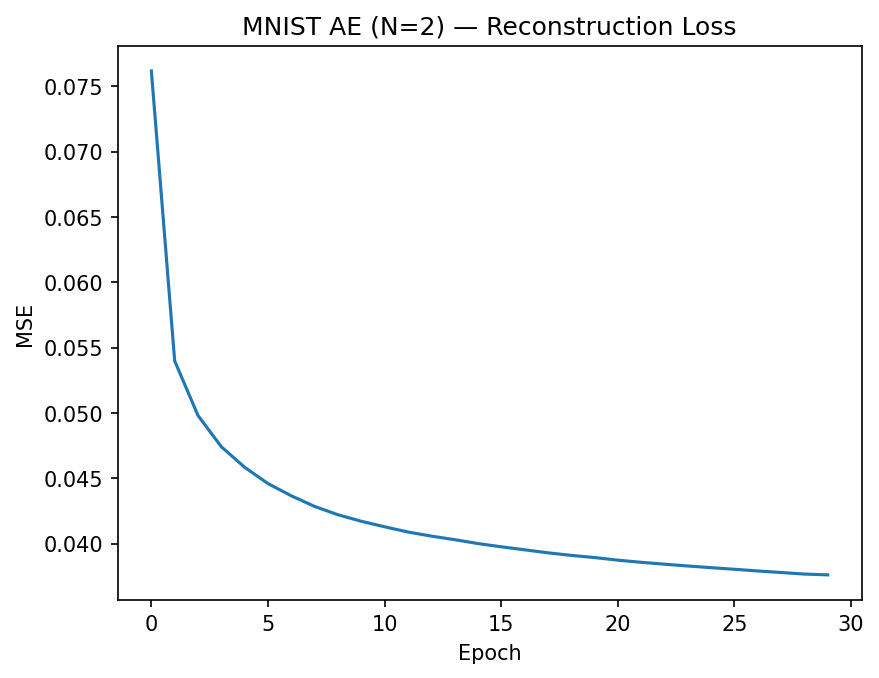
\includegraphics[width=0.7\textwidth]{plots/q31_loss_curve.png}
    \caption{Reconstruction Loss (MSE) over 30 epochs for the MNIST AE with $N=2$.}
    \label{fig:loss}
\end{figure}

\subsection{Original vs Reconstructed Images}
Figure \ref{fig:recon} shows sample test images and their reconstructions. With only 2 latent dimensions, reconstructions are blurry but preserve the overall digit shape.

\begin{figure}[h]
    \centering
    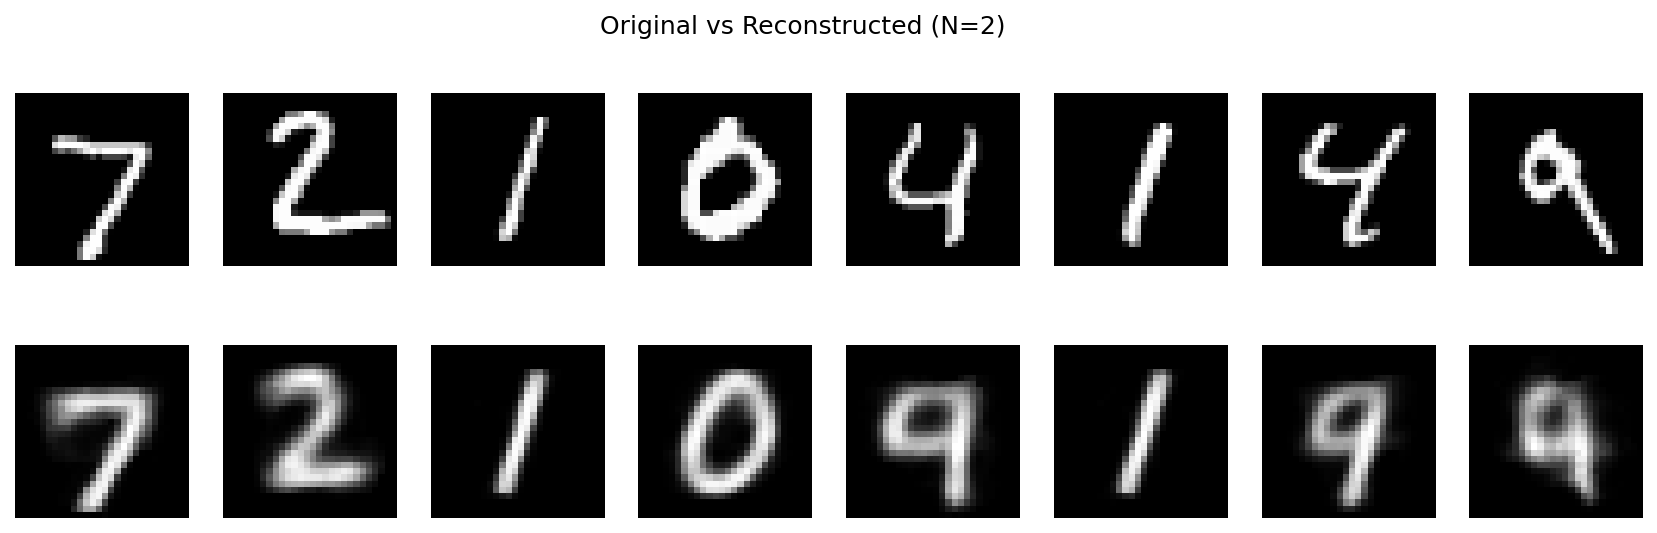
\includegraphics[width=0.85\textwidth]{plots/q31_recon.png}
    \caption{Original (top) vs Reconstructed (bottom) MNIST digits from the $N=2$ Autoencoder.}
    \label{fig:recon}
\end{figure}

\subsection{2D Latent Space Scatter Plot}
Figure \ref{fig:scatter} visualizes the 2D latent codes of the entire MNIST test set, colored by true digit label.

\begin{figure}[h]
    \centering
    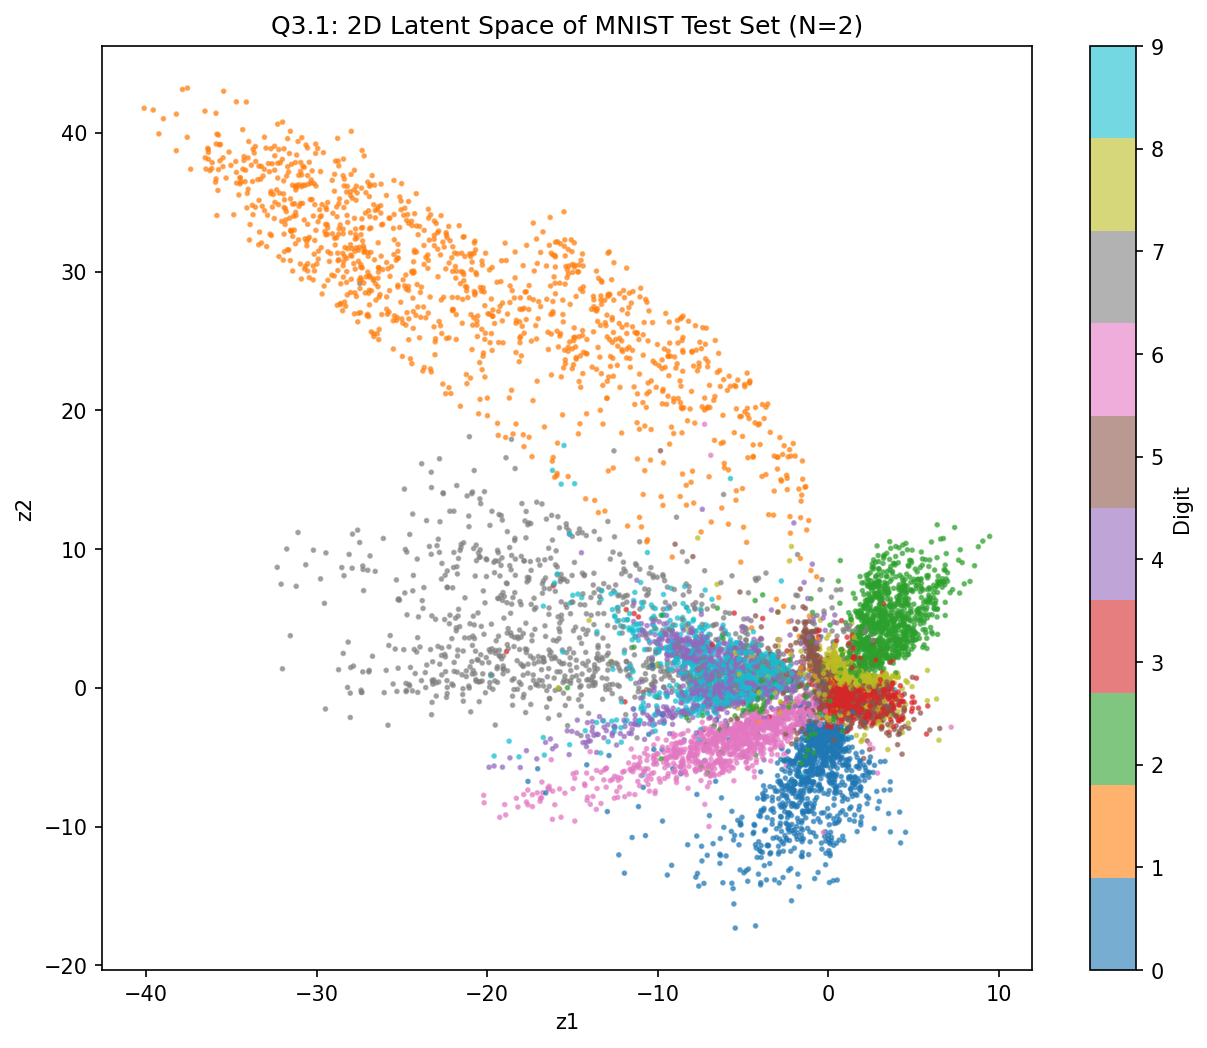
\includegraphics[width=0.85\textwidth]{plots/q31_latent_scatter.png}
    \caption{2D Latent Space of MNIST test set. Each point is an image encoded to 2D, colored by its digit label (0--9).}
    \label{fig:scatter}
\end{figure}

\section{Analysis}
\begin{enumerate}
    \item \textbf{Clustering:} Digits naturally form clusters in the 2D latent space, even though the AE was trained without any label information. This shows the network learns a meaningful representation purely from reconstruction.
    \item \textbf{Similar Digits Overlap:} Visually similar digits (e.g., 4 \& 9, 3 \& 8, 1 \& 7) tend to cluster nearby or partially overlap. This is because they share structural features (e.g., similar stroke patterns), so the encoder maps them to nearby latent coordinates.
    \item \textbf{Distinct Digits Separate:} Structurally distinct digits (e.g., 0 and 1) are well-separated, confirming the latent space captures meaningful visual differences.
\end{enumerate}

\end{document}
